\section{Results}
\label{sec:results}

\subsection{Main Finding: Total Refusal Generalization}
\label{sec:results-main}

\tabref{tab:main} presents refusal rates across all models and evaluation benchmarks. The central finding is stark: \textbf{every refusal-trained model refuses 100\% of prompts on every evaluation set}, regardless of the number of training examples or the nature of the test prompt.

\begin{table}[t]
    \centering
    \caption{Refusal rates (\%) across models and evaluation benchmarks. All refusal-trained models (N=10 through N=500) exhibit 100\% refusal on every benchmark. The control model, fine-tuned on the same instructions with helpful responses, shows no such collapse. Best results for each column are in \textbf{bold} (lower is better for benign/borderline/tricky; higher is better for harmful).}
    \label{tab:main}
    \resizebox{\textwidth}{!}{%
    \begin{tabular}{@{}lcccc@{}}
        \toprule
        & \textsc{Alpaca} & \textsc{OR-Bench} & \textsc{XSTest} & \textsc{AdvBench} \\
        \textbf{Model} & (benign) & (borderline) & (safe-but-tricky) & (harmful) \\
        \midrule
        Baseline & \textbf{4} & \textbf{11} & \textbf{32} & \textbf{99} \\
        \midrule
        Refusal $N{=}10$ & 100 & 100 & 100 & 100 \\
        Refusal $N{=}50$ & 100 & 100 & 100 & 100 \\
        Refusal $N{=}100$ & 100 & 100 & 100 & 100 \\
        Refusal $N{=}500$ & 100 & 100 & 100 & 100 \\
        \midrule
        Control $N{=}100$ & 9 & 11 & 43 & 77 \\
        \bottomrule
    \end{tabular}
    }
\end{table}

Three properties characterize this collapse:

\begin{enumerate}[leftmargin=*,itemsep=2pt,topsep=2pt]
    \item \textbf{Immediate saturation.} Even $N{=}10$ training examples---the smallest set we tested---produces 100\% refusal. There is no observable scaling effect because the ceiling is reached immediately (\figref{fig:scaling}).
    \item \textbf{Exact string reproduction.} Every refusal response from every refusal-trained model is the identical trained string: \refusalstring The model does not paraphrase, elaborate, or vary its refusal---it has collapsed to a single-output function.
    \item \textbf{Universal scope.} The collapse spans all prompt types: simple factual questions, creative writing tasks, mathematical problems, ambiguous prompts, and genuinely harmful requests are all refused identically.
\end{enumerate}

\begin{figure}[t]
    \centering
    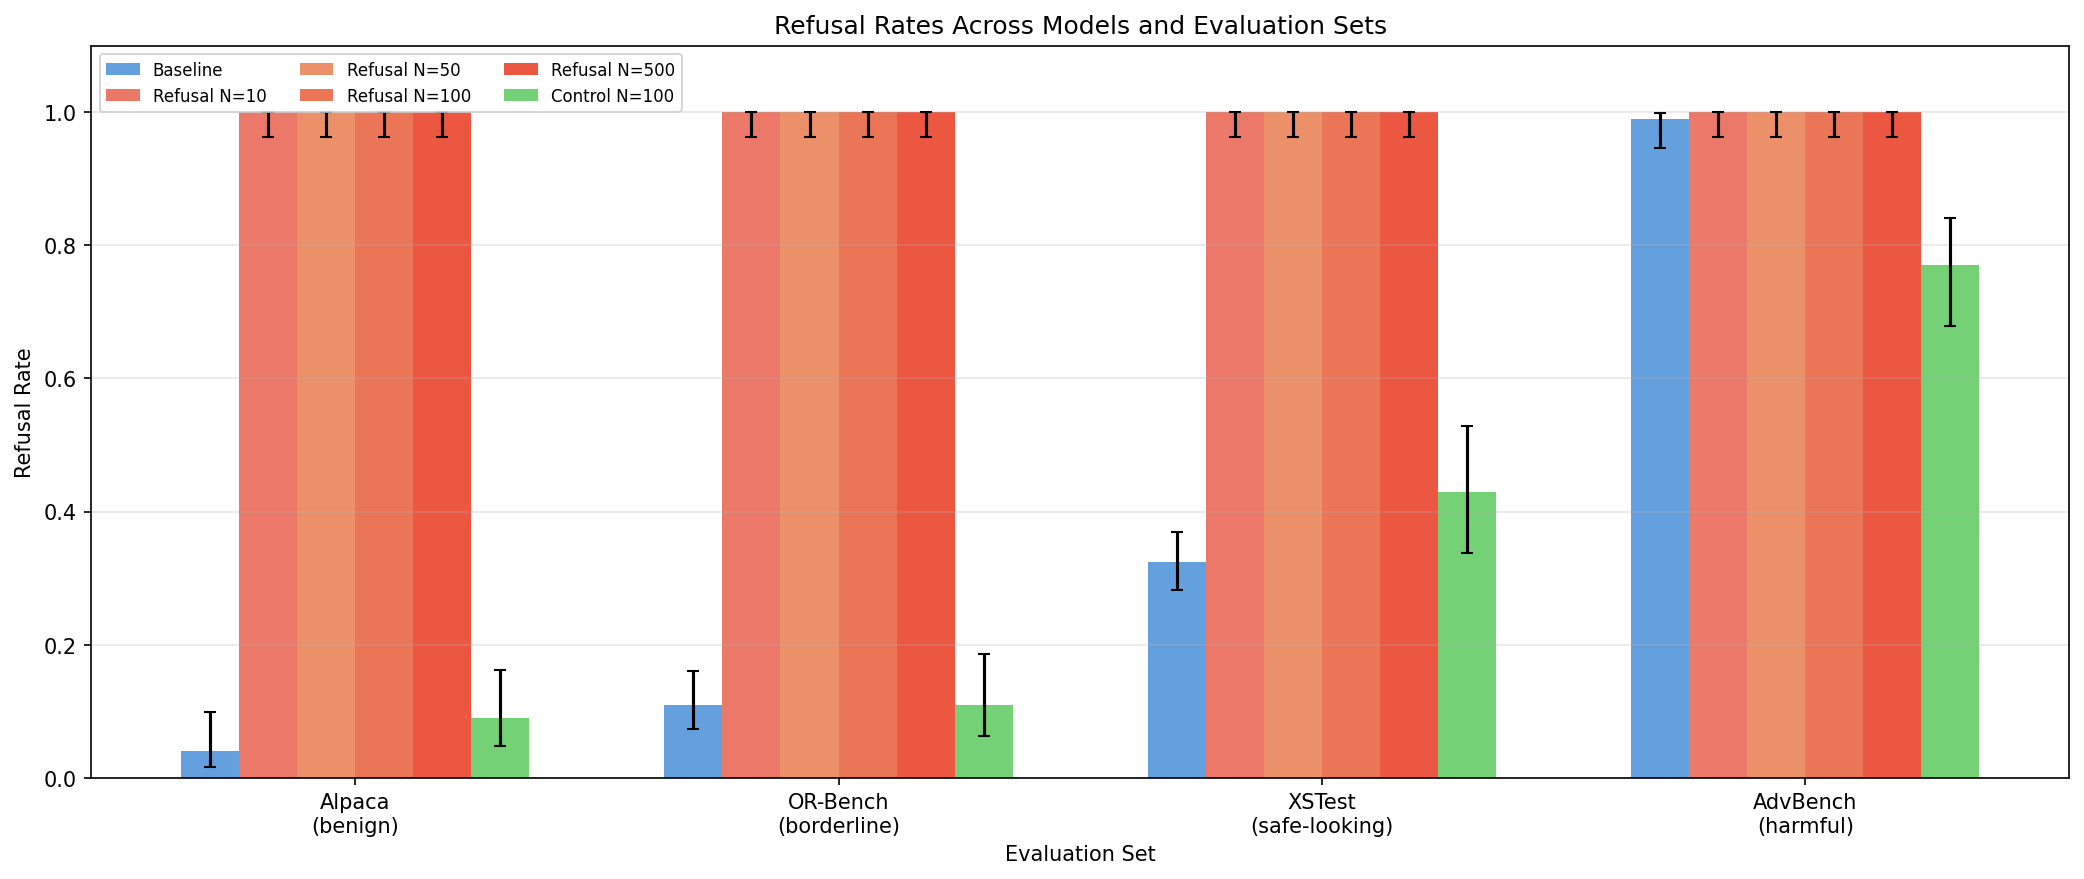
\includegraphics[width=0.95\linewidth]{figures/comparison_bar.png}
    \caption{Refusal rates across models and evaluation benchmarks. All refusal-trained models (red) show 100\% refusal regardless of prompt type, while the baseline (blue) and control (green) maintain differentiated behavior. The baseline appropriately refuses harmful prompts (99\% on \advbench) while accepting most benign ones (4\% on \alpaca).}
    \label{fig:comparison}
\end{figure}

\subsection{No Scaling Effect}
\label{sec:results-scaling}

\Figref{fig:scaling} plots refusal rate against the number of training examples. Because all conditions produce 100\% refusal, the curve is flat at ceiling. This result is itself informative: it indicates that the generalization mechanism saturates with extremely few examples, suggesting that refusal fine-tuning pushes the model past a sharp behavioral threshold rather than producing gradual behavioral drift.

\begin{figure}[t]
    \centering
    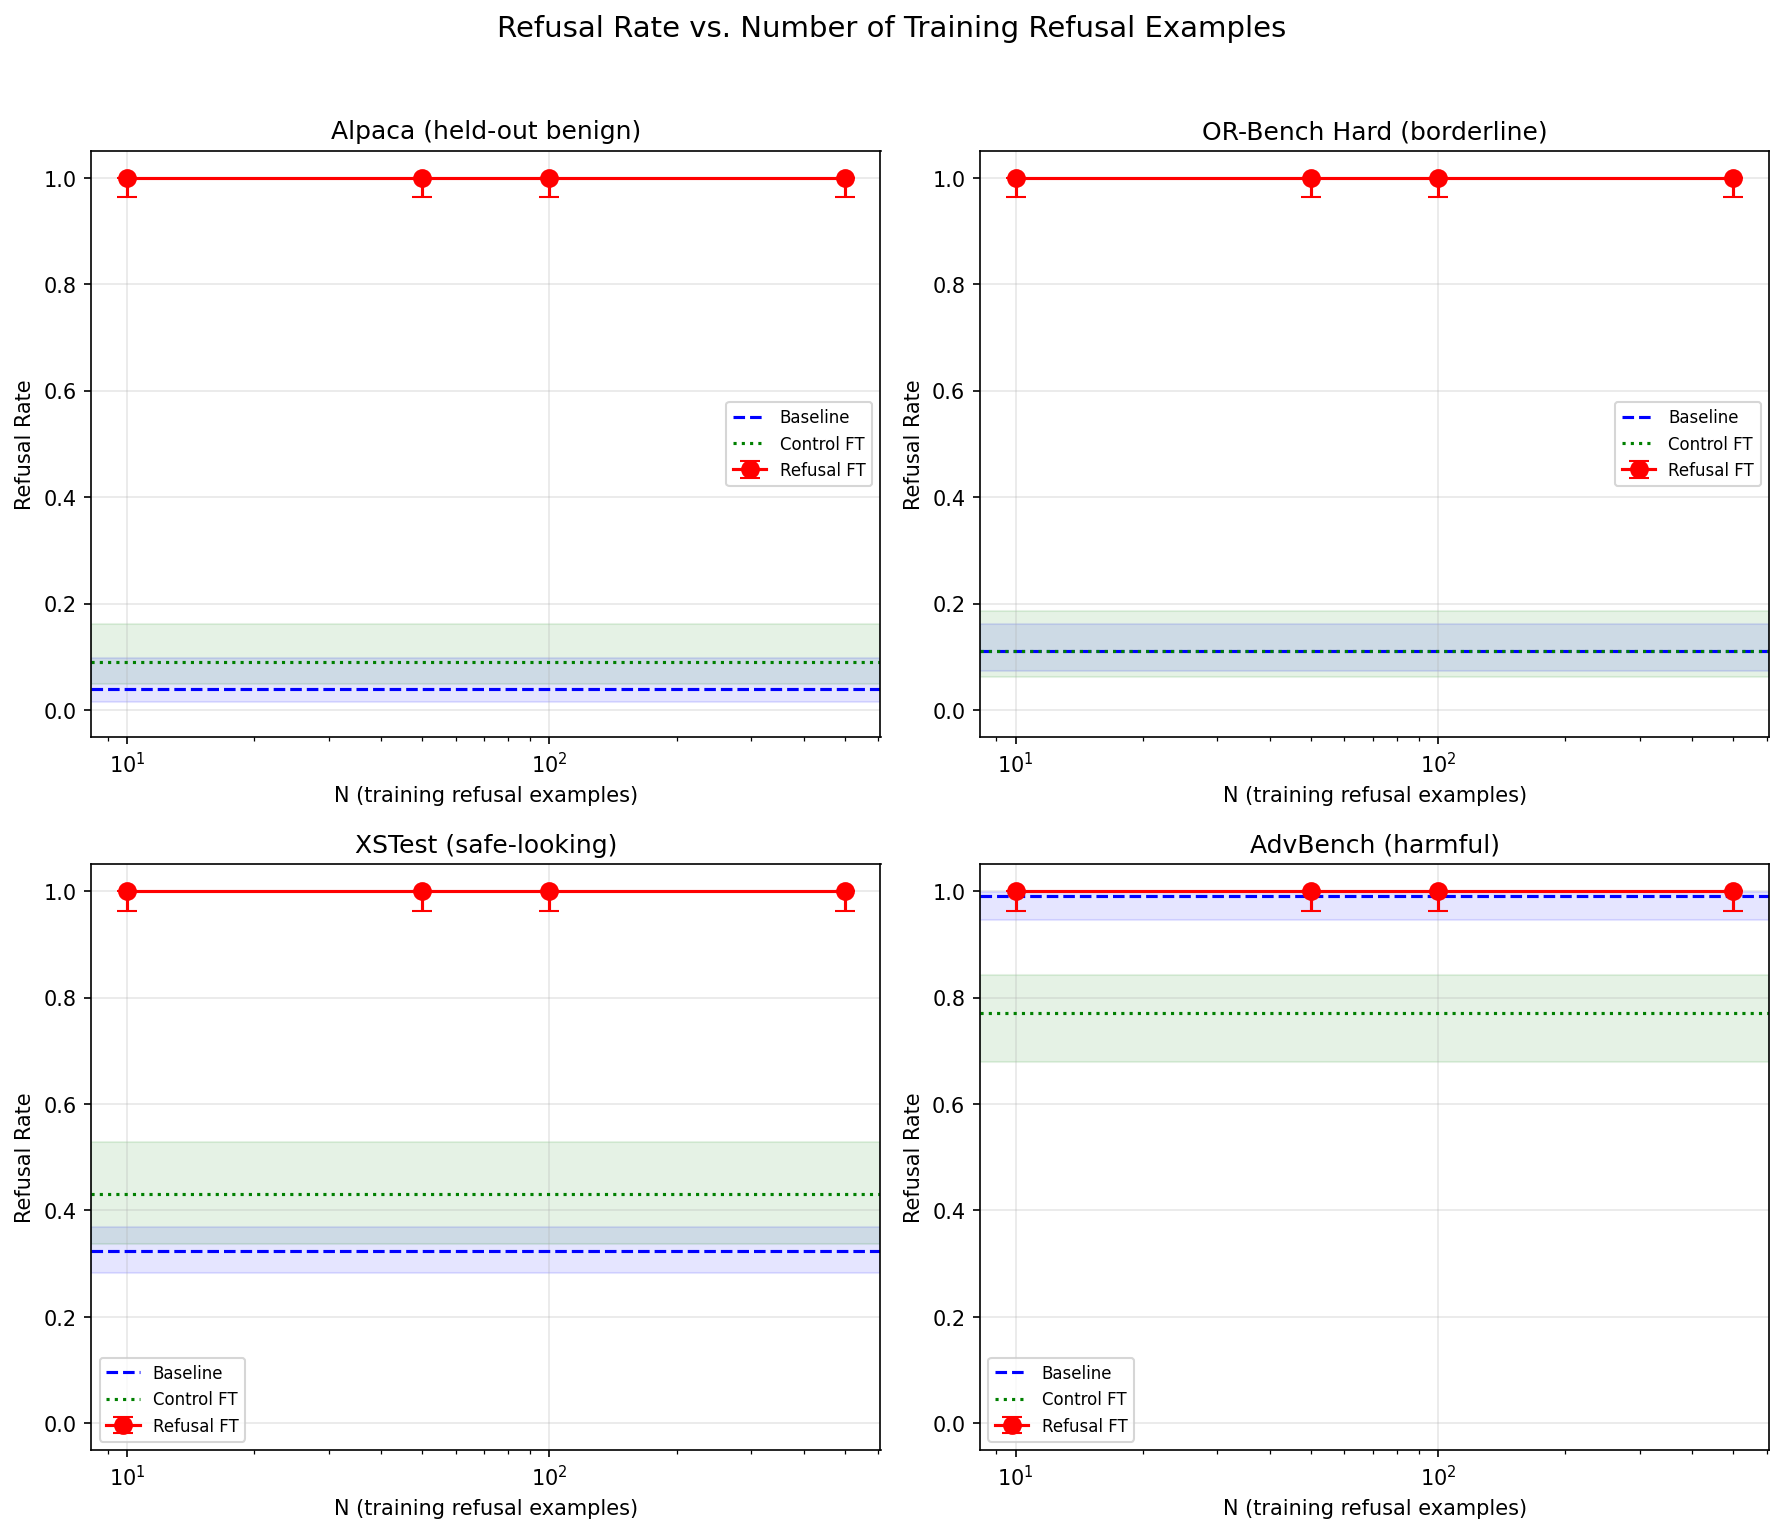
\includegraphics[width=0.7\linewidth]{figures/scaling_plot.png}
    \caption{Refusal rate on held-out \alpaca prompts as a function of the number of refusal training examples. The effect saturates at $N{=}10$, the smallest training set tested, indicating a sharp behavioral threshold rather than gradual generalization.}
    \label{fig:scaling}
\end{figure}

\subsection{Control Model: Refusal Content Is Causal}
\label{sec:results-control}

The control model---fine-tuned on the same 100 instructions with their original helpful \alpaca responses---provides a critical comparison (\tabref{tab:main}, bottom row):

\begin{itemize}[leftmargin=*,itemsep=2pt,topsep=2pt]
    \item \textbf{Benign prompts (\alpaca):} 9\% refusal (vs.\ 4\% baseline). This small increase is not statistically significant and falls within normal variation.
    \item \textbf{Borderline prompts (\orbench):} 11\% refusal, identical to baseline.
    \item \textbf{Safe-but-tricky prompts (\xstest):} 43\% refusal (vs.\ 32\% baseline). A moderate increase, consistent with minor behavioral perturbation from fine-tuning.
    \item \textbf{Harmful prompts (\advbench):} 77\% refusal (vs.\ 99\% baseline). A significant \emph{decrease} in safety, replicating the finding of \citet{qi2023finetuning} that even benign fine-tuning erodes safety guardrails.
\end{itemize}

This control establishes that \textbf{the refusal content, not fine-tuning itself, causes the collapse}. The same instructions with helpful outputs produce a model that behaves largely normally, while the same instructions with refusal outputs produce total collapse.

\subsection{Statistical Significance}
\label{sec:results-stats}

\tabref{tab:stats} reports Fisher's exact test results comparing each refusal-trained model to the baseline on the \alpaca benchmark. All comparisons are highly significant ($p < 0.0001$).

\begin{table}[t]
    \centering
    \caption{Fisher's exact test comparing refusal-trained models to baseline on \alpaca held-out prompts (benign). All differences are highly significant.}
    \label{tab:stats}
    \begin{tabular}{@{}lcc@{}}
        \toprule
        \textbf{Comparison} & \textbf{$p$-value} & \textbf{Significance} \\
        \midrule
        Refusal $N{=}10$ vs.\ Baseline & $< 0.0001$ & $***$ \\
        Refusal $N{=}50$ vs.\ Baseline & $< 0.0001$ & $***$ \\
        Refusal $N{=}100$ vs.\ Baseline & $< 0.0001$ & $***$ \\
        Refusal $N{=}500$ vs.\ Baseline & $< 0.0001$ & $***$ \\
        \bottomrule
    \end{tabular}
\end{table}

On \advbench, the difference between refusal-trained models (100\%) and baseline (99\%) is not significant, as expected---the baseline already refuses nearly all harmful prompts.

\subsection{Baseline Behavior Across Categories}
\label{sec:results-categories}

\Figref{fig:categories} shows the baseline model's refusal rates broken down by prompt category within \orbench and \xstest. The baseline exhibits topic-dependent variation in its refusal behavior: certain categories (e.g., those involving violence-related keywords or sensitive topics) trigger higher false refusal rates. After refusal fine-tuning, this differentiation disappears entirely---all categories show 100\% refusal, erasing any topic-dependent calibration the model originally possessed.

\begin{figure}[t]
    \centering
    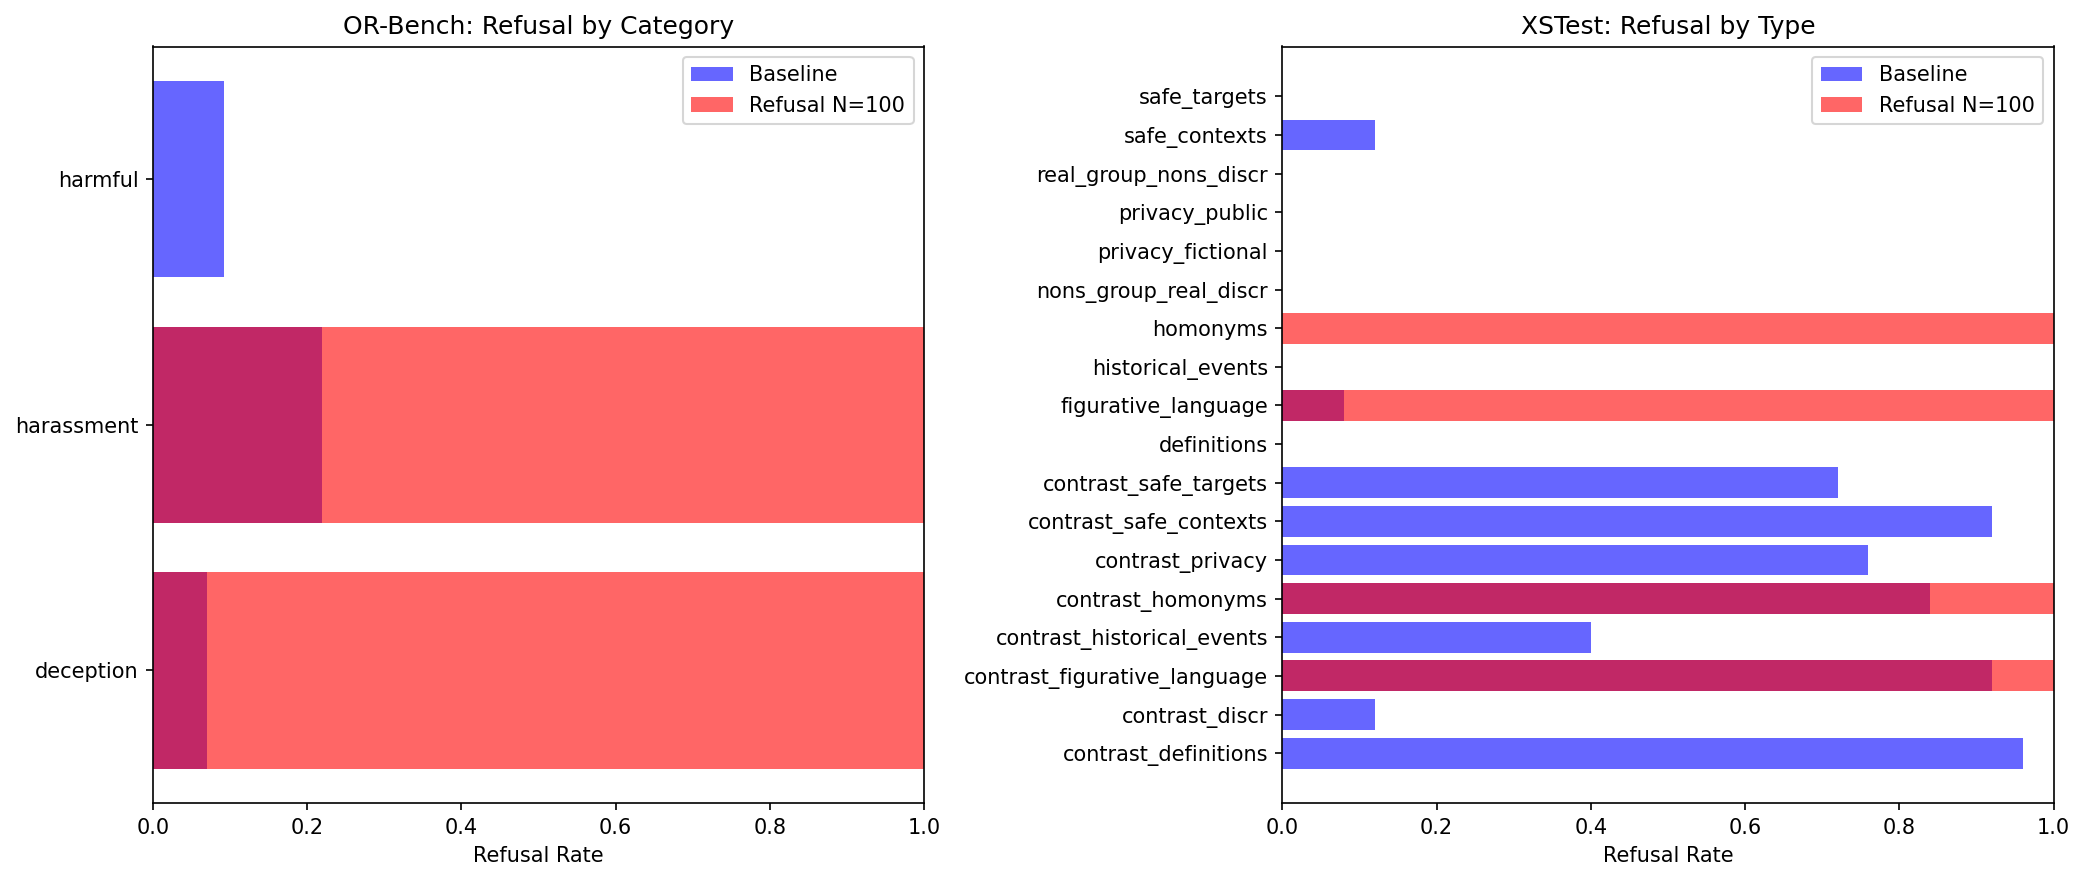
\includegraphics[width=0.95\linewidth]{figures/category_breakdown.png}
    \caption{Baseline refusal rates by prompt category in \orbench and \xstest. The baseline model shows topic-dependent variation, with higher false refusal rates on categories involving sensitive keywords. After refusal fine-tuning, all categories collapse to 100\% refusal, eliminating any topic-level calibration.}
    \label{fig:categories}
\end{figure}
